\documentclass[11pt,landscape]{article}
\usepackage[margin=10mm]{geometry}
\usepackage[T1]{fontenc}
\usepackage[utf8]{inputenc}
\usepackage{lmodern}
\usepackage{amsmath}
\usepackage{amssymb}
\usepackage{tikz}
\usetikzlibrary{arrows.meta, positioning, fit, backgrounds, calc}
\pagestyle{empty}

\begin{document}

\noindent\makebox[\textwidth][c]{\Large GRLNet: Structural Overview}

\vspace{2mm}

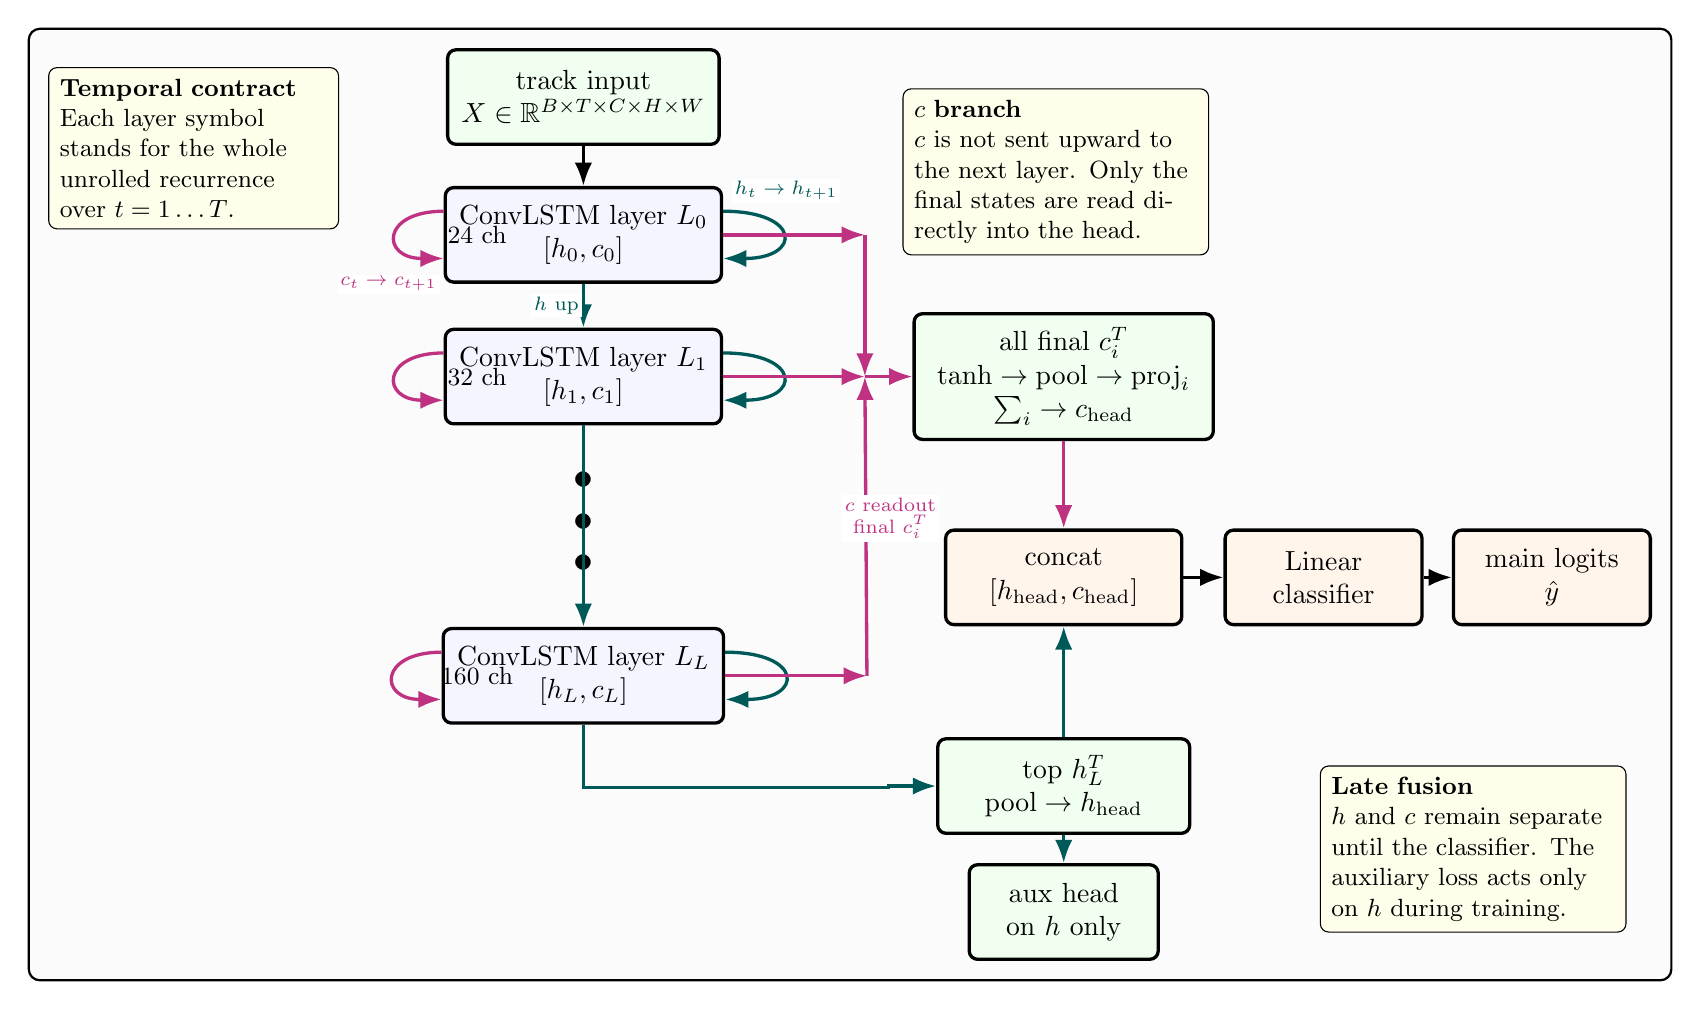
\begin{tikzpicture}[
    >=Latex,
    layer/.style={draw, rounded corners=3pt, very thick, align=center, inner sep=5pt, fill=blue!4, minimum width=30mm, minimum height=12mm},
    io/.style={draw, rounded corners=3pt, very thick, align=center, inner sep=5pt, fill=green!6, minimum width=28mm, minimum height=12mm},
    head/.style={draw, rounded corners=3pt, very thick, align=center, inner sep=5pt, fill=orange!8, minimum width=28mm, minimum height=12mm},
    note/.style={draw, rounded corners=3pt, align=left, inner sep=4pt, fill=yellow!8, text width=34mm, font=\small},
    hpath/.style={->, very thick, draw=teal!70!black},
    tpath/.style={->, very thick, draw=teal!70!black},
    cpath/.style={->, very thick, draw=magenta!75!black},
    main/.style={->, very thick}
]

\node[io, minimum width=34mm] (input) at (4.8,4.55) {
    track input\\
    $X \in \mathbb{R}^{B \times T \times C \times H \times W}$
};

\node[layer] (l0) at (4.8,2.8) {ConvLSTM layer $L_0$\\$[h_0, c_0]$};
\node[layer] (l1) at (4.8,1.0) {ConvLSTM layer $L_1$\\$[h_1, c_1]$};
\node[align=center, font=\Large] at (4.8,-0.85) {$\bullet$\\[-3pt]$\bullet$\\[-3pt]$\bullet$};
\node[layer] (lL) at (4.8,-2.8) {ConvLSTM layer $L_L$\\$[h_L, c_L]$};

\node[font=\small] at (3.45,2.8) {$24$ ch};
\node[font=\small] at (3.45,1.0) {$32$ ch};
\node[font=\small] at (3.45,-2.8) {$160$ ch};

\draw[main] (input.south) -- (l0.north);
\draw[hpath] (l0.south) -- node[left, font=\scriptsize, text=teal!70!black, fill=white, inner sep=1pt] {$h$ up} (l1.north);
\draw[hpath] (l1.south) -- (lL.north);

\draw[tpath] ($(l0.east)+(0mm,3mm)$) .. controls +(10mm,0) and +(10mm,0) .. ($(l0.east)+(0mm,-3mm)$);
\draw[tpath] ($(l1.east)+(0mm,3mm)$) .. controls +(10mm,0) and +(10mm,0) .. ($(l1.east)+(0mm,-3mm)$);
\draw[tpath] ($(lL.east)+(0mm,3mm)$) .. controls +(10mm,0) and +(10mm,0) .. ($(lL.east)+(0mm,-3mm)$);
\node[anchor=south, font=\scriptsize, text=teal!70!black, fill=white, inner sep=1pt] at ($(l0.east)+(8mm,4mm)$) {$h_t \rightarrow h_{t+1}$};

\draw[cpath] ($(l0.west)+(0mm,3mm)$) .. controls +(-8mm,0) and +(-8mm,0) .. ($(l0.west)+(0mm,-3mm)$);
\draw[cpath] ($(l1.west)+(0mm,3mm)$) .. controls +(-8mm,0) and +(-8mm,0) .. ($(l1.west)+(0mm,-3mm)$);
\draw[cpath] ($(lL.west)+(0mm,3mm)$) .. controls +(-8mm,0) and +(-8mm,0) .. ($(lL.west)+(0mm,-3mm)$);
\node[anchor=north, font=\scriptsize, text=magenta!75!black, fill=white, inner sep=1pt] at ($(l0.west)+(-7mm,-5mm)$) {$c_t \rightarrow c_{t+1}$};

\draw[cpath] (l0.east) -- ++(18mm,0);
\draw[cpath] (l1.east) -- ++(18mm,0);
\draw[cpath] (lL.east) -- ++(18mm,0);
\draw[cpath, very thick] ($(l0.east)+(18mm,0)$) -- ($(l1.east)+(18mm,0)$);
\draw[cpath, very thick] ($(lL.east)+(18mm,0)$) -- ($(l1.east)+(18mm,0)$);
\node[font=\scriptsize, text=magenta!75!black, fill=white, inner sep=1pt, align=center] at (8.7,-0.8) {$c$ readout\\final $c_i^T$};

\node[io, minimum width=38mm] (cread) at (10.9,1.0) {
    all final $c_i^T$\\
    $\tanh \rightarrow \mathrm{pool} \rightarrow \mathrm{proj}_i$\\
    $\sum_i \rightarrow c_{\mathrm{head}}$
};
\draw[cpath] ($(l1.east)+(18mm,0)$) -- (cread.west);

\node[io, minimum width=32mm] (hread) at (10.9,-4.20) {
    top $h_L^T$\\
    $\mathrm{pool} \rightarrow h_{\mathrm{head}}$
};
\draw[hpath] (lL.south) -- ++(0,-8mm) -| ($(hread.west)+(-6mm,0)$) -- (hread.west);

\node[head, minimum width=30mm] (concat) at (10.9,-1.55) {
    concat\\
    $[h_{\mathrm{head}}, c_{\mathrm{head}}]$
};
\draw[hpath] (hread.north) -- (concat.south);
\draw[cpath] (cread.south) -- (concat.north);

\node[head, minimum width=25mm] (fc) at (14.2,-1.55) {Linear\\classifier};
\node[head, minimum width=25mm] (out) at (17.1,-1.55) {main logits\\$\hat{y}$};
\draw[main] (concat.east) -- (fc.west);
\draw[main] (fc.east) -- (out.west);

\node[io, minimum width=24mm] (aux) at (10.9,-5.8) {
    aux head\\
    on $h$ only
};
\draw[dashed, ->, very thick, draw=teal!70!black] (hread.south) -- (aux.north);

\node[note] (n1) at (-0.15,3.9) {
\textbf{Temporal contract}\\
Each layer symbol stands for the whole unrolled recurrence over
$t=1 \dots T$.
};

\node[note, text width=36mm] (n2) at (10.8,3.6) {
\textbf{$c$ branch}\\
$c$ is not sent upward to the next layer. Only the final states are read directly into the head.
};

\node[note, text width=36mm] (n3) at (16.1,-5.0) {
\textbf{Late fusion}\\
$h$ and $c$ remain separate until the classifier. The auxiliary loss acts only on $h$ during training.
};

\begin{scope}[on background layer]
    \node[draw, rounded corners=4pt, thick, fit=(input)(l0)(l1)(lL)(cread)(hread)(concat)(fc)(out)(aux)(n1)(n2)(n3), inner sep=7pt, fill=gray!3] {};
\end{scope}

\end{tikzpicture}

\end{document}
